\documentclass{beamer}
\usepackage[utf8]{inputenc}

\usepackage{amsmath}
\usepackage{graphicx}
\usepackage{url}
\usepackage{fancyvrb}
\usepackage{xcolor}

\usetheme{Madrid}
\usecolortheme{seahorse}

\usepackage{inconsolata}
\usepackage[scaled]{helvet}
\renewcommand*\familydefault{\sfdefault}
\usepackage[T1]{fontenc}

\usepackage{listings}
\usepackage{color}

\definecolor{codegreen}{rgb}{0,0.6,0}
\definecolor{codegray}{rgb}{0.5,0.5,0.5}
\definecolor{codepurple}{rgb}{0.58,0,0.82}
\definecolor{backcolour}{rgb}{0.95,0.95,0.92}

\mode<presentation>

\definecolor{orange}{HTML}{BC2E07}

\usepackage{hyperref}
\hypersetup{
    colorlinks,
    linkcolor=orange,
    urlcolor=blue
}

\lstdefinestyle{mystyle}{
    language=C++,
    basicstyle=\ttfamily\footnotesize,
    backgroundcolor=\color{backcolour},
    commentstyle=\color{codegreen},
    keywordstyle=\color{magenta},
    numberstyle=\tiny\color{codegray},
    stringstyle=\color{codepurple},
    breakatwhitespace=false,
    breaklines=true,
    captionpos=b,
    keepspaces=true,
    numbers=left,
    numbersep=5pt,
    showspaces=false,
    showstringspaces=false,
    showtabs=false,
    tabsize=2
}

\title{Lab \# 9: Structures}
\subtitle{EC-102 -- Computer Systems and Programming}

\author{Usman Ayub Sheikh}
\institute{School of Mechanical and Manufacturing Engineering (SMME), \\ National University of Sciences and Technology (NUST)}
\date{\today}

\begin{document}
\begin{frame}
    \titlepage
\end{frame}

\begin{frame}
    \frametitle{Outline}
        \tableofcontents
\end{frame}

\begin{frame}
    \frametitle{Structures -- Why?}
    \section{Structures} % (fold)
    \label{sec:structures}
    \subsection{Why?} % (fold)
    \label{sub:why}
    \begin{itemize}
        \item Variables of such data types as \texttt{int}, \texttt{float} and \texttt{char} can represent, at most, one item of information e.g. a length or a width
        \item In the physical world, we deal with entities such as people and cars, all with their own set of attributes/characteristics such as name, size and weight etc.
        \item In order to model such things, we want to be able to not only
        \begin{itemize}
            \item group all the relevant data of an entity into a single variable, but also
            \item work with that variable as we work with variables of type \texttt{int} or \texttt{float}
        \end{itemize}
    \end{itemize}
\end{frame}

\begin{frame}
    \frametitle{Structures -- Why?}
    \begin{figure}
        \centering
        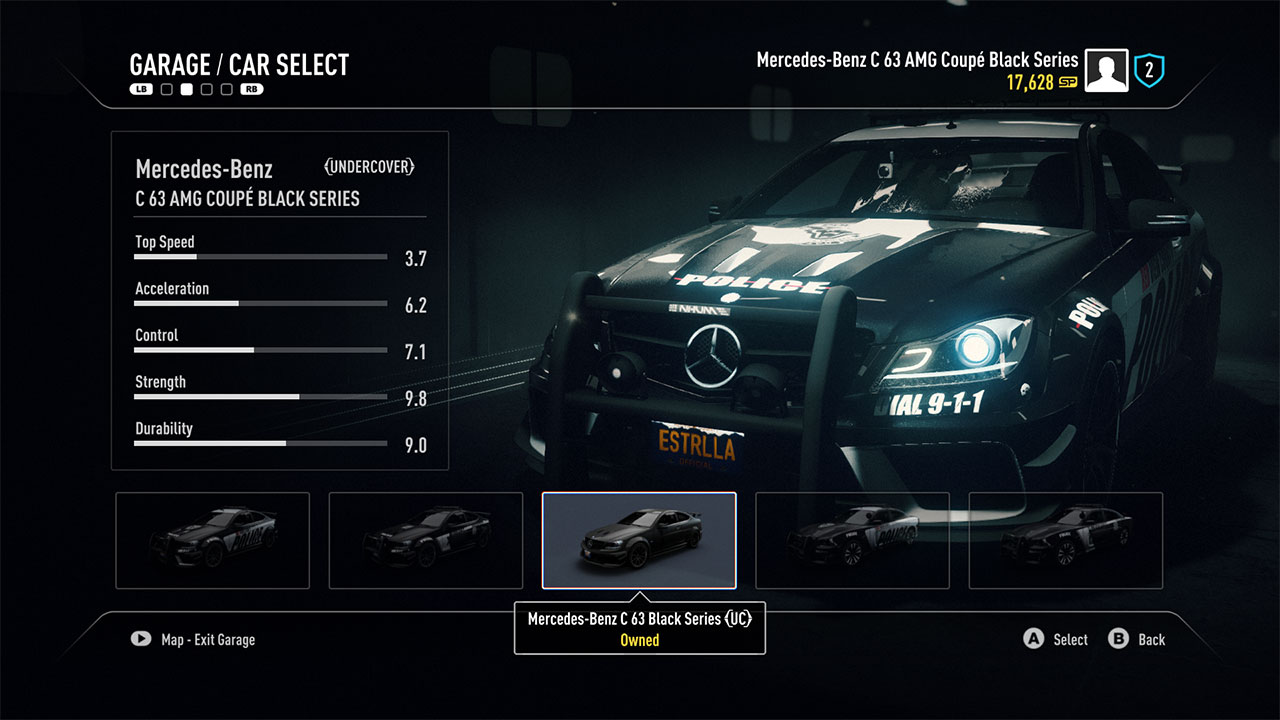
\includegraphics[scale=0.265]{car_select.jpg}
    \end{figure}
\end{frame}

\begin{frame}
    \frametitle{Structures -- Why?}
    \begin{figure}
        \centering
        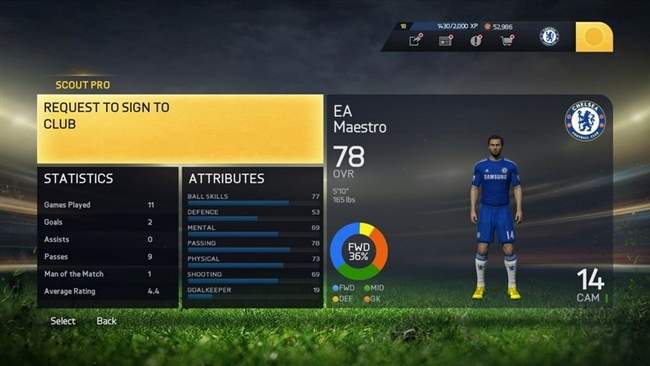
\includegraphics[scale=0.7]{player_select.jpg}
    \end{figure}
\end{frame}

\begin{frame}
    \frametitle{Structures -- What?}
    \subsection{What?} % (fold)
    \label{sub:what}
    \begin{itemize}
        \item A \textbf{collection} of simple variables
        \item The variables can be of \textbf{different} types, and
        \item Are known as the \textbf{members} of the structure
        \item Examples:
        \begin{itemize}
            \item An item in a widget company's parts inventory
            \begin{itemize}
                \item Model number
                \item ID
                \item Cost
            \end{itemize}
            \item A student of BS Mechanical Engineering
            \begin{itemize}
                \item Name
                \item Reg. No.
                \item Section
            \end{itemize}
        \end{itemize}
    \end{itemize}
\end{frame}

\begin{frame} [fragile]
    \frametitle{Structures -- How?}
    \subsection{How?} % (fold)
    \label{sub:how}
    \subsubsection{A Simple Structure} % (fold)
    \label{subsubsec:a_simple_structure}
    \lstset{style=mystyle}
    \begin{lstlisting}
#include <iostream>
using namespace std;

struct part
{
    int id;
    float cost;
};

int main()
{
    part part1;

    part1.id = 12;
    part1.cost = 22.57;

    cout << "ID " << part1.id << " Cost " << part1.cost;
    return 0;
}
\end{lstlisting}
\end{frame}

\begin{frame}[fragile]
    \frametitle{Defining the Structure}
    \subsubsection{Defining the Structure} % (fold)
    \label{ssub:defining_the_structure}
    \begin{columns}
        \column{0.4\textwidth}
        \lstset{style=mystyle}
\begin{lstlisting}
struct part
{
    int id;
    float cost;
};
\end{lstlisting}
        \column{0.57\textwidth}
            \begin{itemize}
            \item The keyword \texttt{struct} introduces the structure definition
            \item Next comes the structure name
            \item The declarations of the structure members -- id and cost -- are enclosed in braces
            \item A semicolon follows the closing brace, terminating the entire structure
            \end{itemize}
    \end{columns}
\end{frame}

\begin{frame}[fragile]
    \frametitle{Defining the Structure}
    \begin{columns}
        \column{0.4\textwidth}
        \lstset{style=mystyle}
\begin{lstlisting}
struct part
{
    int id;
    float cost;
};
\end{lstlisting}
        \column{0.57\textwidth}
            \begin{itemize}
            \item The structure definition serves \textbf{only} as a blueprint for the creation of variables of type \texttt{part}
            \item Unlike the definition of a simple variable, it does not set aside any memory or even name any variables
            \item It is merely a specification of how structure variables will look when they are defined
            \end{itemize}
    \end{columns}
\end{frame}

\begin{frame}[fragile]
    \frametitle{Defining Structure Variables}
    \subsubsection{Defining Structure Variables} % (fold)
    \label{ssub:defining_structure_variables}
    \begin{columns}
        \column{0.4\textwidth}
        \lstset{style=mystyle}
\begin{lstlisting}
part part1;
part part2;
part part3;
\end{lstlisting}
        \column{0.57\textwidth}
            \begin{itemize}
            \item Line 1 defines a variable \texttt{part1} of type structure \texttt{part}, Line 2 and 3 define a few more variables of the same type
            \item These definitions reserve space in the memory for \texttt{part1}, \texttt{part2} and \texttt{part3} respectively
            \item How much space for \texttt{part1}? Enough to hold all the members i.e. \texttt{id} and \texttt{cost}
            \item 4 bytes for the \texttt{id} and 4 bytes for the \texttt{cost} = 8 bytes for one \texttt{part} variable
            \end{itemize}
    \end{columns}
\end{frame}

\begin{frame}[fragile]
    \frametitle{Accessing Structure Members}
    \subsubsection{Accessing Structure Members} % (fold)
    \label{ssub:accessing_structure_members}
    \begin{columns}
        \column{0.4\textwidth}
        \lstset{style=mystyle}
\begin{lstlisting}
part1.id = 22;
part2.id = 23;
part3.id = 24;

part1.cost = 45.55;
part2.cost = 34.64;
part3.cost = 24.55;
\end{lstlisting}
        \column{0.57\textwidth}
            \begin{itemize}
            \item Once a structure has been defined, its members can be accessed using a \textbf{dot operator}
            \item The structure member is written in three parts:
            \begin{enumerate}
                \item the name of the structure variable e.g. \texttt{part1},
                \item the dot operator, and
                \item the member name e.g. \texttt{id}
            \end{enumerate}
            \item \texttt{part3.id} means the \texttt{id} member of \texttt{part3}
            \end{itemize}
    \end{columns}
\end{frame}

\begin{frame}[fragile]
    \frametitle{Accessing Structure Members}
    \begin{columns}
        \column{0.4\textwidth}
        \lstset{style=mystyle}
\begin{lstlisting}
cout << "IDs: " << endl;
cout << part1.id << endl;
cout << part2.id << endl;
cout << part3.id << endl;

\end{lstlisting}
        \column{0.57\textwidth}
            \begin{itemize}
            \item Structure members are treated just like other variables
            \item In the assignment statement \texttt{part1.id = 22}, the \texttt{id} member of \texttt{part1} has been assigned a value of 22
            \item Similarly, \texttt{cout} statements can be used to display the \texttt{id} of each of the three parts
            \end{itemize}
    \end{columns}
\end{frame}

\begin{frame} [fragile]
\frametitle{Other Structure Features}
\section{Other Structure Features} % (fold)
\label{sec:other_structure_features}
    \begin{itemize}
        \item Structure members can be \textbf{initialized} when the structure variable is defined
        \lstset{style=mystyle}
\begin{lstlisting}
    part part1 = {22, 45.55};
    part part2 = {23, 34.64};
    part part3 = {24, 24.55};

\end{lstlisting}
        \item One structure variable can be \textbf{assigned} to another variable of the same type as follows:
        \lstset{style=mystyle}
\begin{lstlisting}
    part1 = part2;

\end{lstlisting}
The value of each member of \texttt{part2} is assigned to the corresponding member of \texttt{part1}
    \end{itemize}
\end{frame}

\begin{frame} [fragile]
    \frametitle{Solved Example 1}
    \section{Solved Examples} % (fold)
    \label{sec:solved_examples}
    \subsection{Solved Example 1} % (fold)
    \label{sub:solved_example_1}
    \lstset{style=mystyle}
\begin{lstlisting}
// demonstrates some additional features of structures
#include <iostream>
using namespace std;

struct part
{
    int modelnumber;
    int partnumber;
    float cost;
};

int main()
{
    part part1 = {6244, 373, 217.55F};
    part part2;

    cout << "Model " << part1.modelnumber;
    cout << ", part " << part1.partnumber;
    cout << ", cost $" << part1.cost << endl;

\end{lstlisting}
\end{frame}

\begin{frame} [fragile]
    \frametitle{Solved Example 1}
    \lstset{style=mystyle}
\begin{lstlisting} [firstnumber=20]
    part2 = part1;

    cout << "Model " << part2.modelnumber;
    cout << ", part " << part2.partnumber;
    cout << ", cost $" << part2.cost << endl;

    return 0;
}
\end{lstlisting}
\end{frame}

\begin{frame} [fragile]
    \frametitle{Solved Example 2}
    \subsection{Solved Example 2} % (fold)
    \label{sub:solved_example_2}
    \lstset{style=mystyle}
\begin{lstlisting}
// demonstrates structures using English measurements
#include <iostream>
using namespace std;

struct Distance
{
    int feet;
    float inches;
};

int main()
{
    Distance d1, d3;
    Distance d2 = {11, 6.25};

    cout << "\nEnter feet: ";
    cin >> d1.feet;
    cout << "Enter inches: ";
    cin >> d1.inches;

\end{lstlisting}
\end{frame}

\begin{frame} [fragile]
    \frametitle{Solved Example 2}
    \lstset{style=mystyle}
\begin{lstlisting} [firstnumber=20]
    d3.inches = d1.inches + d2.inches;
    d3.feet = 0;

    if(d3.inches >= 12.0)
    {
        d3.inches -= 12.0;
        d3.feet++;
    }
    d3.feet += d1.feet + d2.feet;

    cout << d1.feet << "\'-" << d1.inches << "\" + ";
    cout << d2.feet << "\'-" << d2.inches << "\" = ";
    cout << d3.feet << "\'-" << d3.inches << "\"\n";

    return 0;
}
\end{lstlisting}
\end{frame}

\begin{frame} [fragile]
    \frametitle{Solved Example 3}
    \subsection{Solved Example 3} % (fold)
    \label{sub:solved_example_3}
    \lstset{style=mystyle}
\begin{lstlisting}
// demonstrates structures within structures
#include <iostream>
using namespace std;

struct Distance
{
    int feet;
    float inches;
};

struct Room
{
    Distance length;
    Distance width;
};

\end{lstlisting}
\end{frame}

\begin{frame} [fragile]
    \frametitle{Solved Example 3}
    \lstset{style=mystyle}
\begin{lstlisting} [firstnumber=16]
int main()
{
    Room dining;

    dining.length.feet = 13; // nested structure member
    dining.length.inches = 6.5;
    dining.width.feet = 10;
    dining.width.inches = 0.0;

    float l = dining.length.feet + dining.length.inches / 12;
    float w = dining.width.feet + dining.width.inches / 12;

    cout << "Dining room area is: " << l * w << " sq ft\n";
    return 0;
}
\end{lstlisting}
\end{frame}

\begin{frame}
    \frametitle{Exercise 1}
    \section{Exercises} % (fold)
    \label{sec:exercises}
    \subsection{Exercise 1} % (fold)
    \label{sub:exercise_1}
    \begin{itemize}
        \item Create a structure called \texttt{employee} that contains two members:
        \begin{itemize}
            \item an employee number (type \texttt{int}), and
            \item the employee's compensation (in dollars, type \texttt{float})
        \end{itemize}
        \item Ask the user to fill in this data for three employees
        \item Store it in three variables of type \texttt{struct} \texttt{employee}, and then
        \item Display the information for each employee
    \end{itemize}
\end{frame}

\begin{frame}
    \frametitle{Exercise 2}
    \subsection{Exercise 2} % (fold)
    \label{sub:exercise_2}
    \begin{itemize}
        \item Create a structure called \texttt{Volume} that uses three variables of type \texttt{Distance} to model the volume of a room.
        \item Initialize a variable of type \texttt{Volume} to specific dimensions, then,
        \item Calculate the volume it represents, and
        \item Print out the result
    \end{itemize}
\end{frame}
\end{document}
